\hypertarget{concurrent-repair-at-106-sites-many-units-against-one}{%
\chapter{Concurrent repair at 10\^{}\label{doc:concurrency}6 sites: many units against
one}\label{concurrency-concurrent-repair-at-106-sites-many-units-against-one}}

Module 29. Code: \texttt{scripts/m29\_concurrency.py} (reusing
\texttt{picsim/megasort.py} and the settings of module 28); results
\texttt{results/m29\_capacity.json}, \texttt{results/m29\_ladder.json},
\texttt{results/m29\_hardware.json}, \texttt{results/m29\_figure.png}.
Values are SIM or DERIVED, valid in the regime stated, and should be
reviewed before they are quoted.

\hypertarget{1-result}{%
\section{Result}\label{concurrency-1-result}}

The proposition tested comes from the analysis that followed module 28.
It holds that steady-state repair at 10\^{}6 sites is limited per
stream, so the winning quantity is the number of engines working at
once, and that chips replicate where AOD pairs do not. In our model the
first half holds and the second does not.

(i) \textbf{Concurrency is needed at 10\^{}6 sites, by every method.}
One unit scanning the whole array leaves the array at a time-averaged
defect fraction of 8.9e-4 (PIC 32 x 4, 128 engines) to 6.2e-3 (crossed
AOD with a 40-site field) with tau = 3000 s. Four units bring every
method to 1.66e-4 to 1.68e-4, and sixteen to 1.37e-4 to 1.39e-4, close
to the floor eps + T/(2 tau) = 1.17e-4.

(ii) \textbf{Concurrency does not favour the PIC.} At equal K the units
converge. Every unit needs K = 4 for 2e-4 and K = 16 for 1.5e-4, and
with K = 16 even a single moving tweezer per zone holds 1.37e-4. The PIC
units then cost far more. Fast control channels are the fixed cost;
laser power is given provisioned and in steady state:

{\footnotesize
\begin{longtable}[]{@{}>{\raggedright\arraybackslash}p{0.229\dimexpr(\linewidth-12\tabcolsep)\relax}>{\raggedright\arraybackslash}p{0.145\dimexpr(\linewidth-12\tabcolsep)\relax}>{\raggedright\arraybackslash}p{0.122\dimexpr(\linewidth-12\tabcolsep)\relax}>{\raggedright\arraybackslash}p{0.168\dimexpr(\linewidth-12\tabcolsep)\relax}>{\raggedright\arraybackslash}p{0.145\dimexpr(\linewidth-12\tabcolsep)\relax}>{\raggedright\arraybackslash}p{0.191\dimexpr(\linewidth-12\tabcolsep)\relax}@{}}
\toprule\noalign{}
K & PIC 32 x 4 & PIC 16 x 1 & AOD, 128-site field & AOD, 40-site field &
single tweezer \\
\midrule\noalign{}
\endhead
\bottomrule\noalign{}
\endlastfoot
4 (\textless= 2e-4): channels & 196,096 & 24,512 & 8 & 8 & not
simulated \\
power provisioned / steady & 71.5 W / 0.25 W & 40.6 W / 0.23 W & 9.0 W /
0.076 W & 3.0 W / 0.075 W & \\
16 (\textless= 1.5e-4): channels & 784,384 & 98,048 & 32 & 32 & 32 \\
power provisioned / steady & 286 W / 0.99 W & 162 W / 0.94 W & 36 W /
0.30 W & 12 W / 0.30 W & 0.30 W / 0.30 W \\
\end{longtable}
}

K counts whole units, ceil(10\^{}6 / sites per zone). Transport laser
power is at 1.2 mK; divide by 4 for the 0.3 mK moving depth of the
transport model.

\begin{itemize}
\tightlist
\item
  \textbf{Provisioned power} covers each unit at its peak simultaneous
  tweezers when busy (assembly or saturation, up to 310 for PIC 32 x 4).
\item
  \textbf{Steady-state power} is K x the mean tweezers per pass in the
  steady window, about 1.0 to 1.1 per unit. (Corrected: an earlier
  version used the non-integer 10\^{}6 / sites per zone, which gave
  slightly low totals, e.g. 195,705 instead of 196,096, and showed only
  the provisioned power.)
\end{itemize}

(iii) \textbf{Throughput is not the limit.} At saturation, the capacity
per unit with cold steps is:

\begin{itemize}
\tightlist
\item
  PIC 32 x 4: about 76,000 moves/s;
\item
  PIC 16 x 1 and the 128-site AOD: about 37,000 to 40,000;
\item
  40-site AOD: about 20,000;
\item
  single tweezer: 570. The demand at 10\^{}6 sites is 1,242/s at tau
  3000 s and 4,242/s at 300 s, with the simulator\textquotesingle s
  image cycle T\_img + t\_img = 0.11 s. The measured refill rates match:
  1,225/s and 4,247/s for PIC 32 x 4 at K = 1. (Corrected: an earlier
  version used a 0.1 s cycle, 1,335/s and 4,330/s.) What limits one unit
  on a large array is latency: the time its field needs to come back to
  a new hole after each image. Splitting the array shortens that time
  for every method alike.
\end{itemize}

The analysis\textquotesingle s starting figure, 420 to 570 refills/s
"per stream", was measured for the single tweezer only. For the other
units, module 28 measured the refill rate equal to the demand, not their
capacity.

By the decision rule set before the runs, the PIC unit needs as many
units (beam paths into the objective) as AOD pairs for the same target,
with more power and channels. Concurrency therefore does not make the
case for PIC transport. The case for it rests on assembly speed from a
random loading (module 28).

\hypertarget{2-method}{%
\section{Method}\label{concurrency-2-method}}

Zones are independent, since each holds its own reservoir rows and its
own unit. K units on 10\^{}6 sites are therefore one zone of 10\^{}6 / K
computation sites, simulated with the units and settings of module 28.
Those are:

\begin{itemize}
\tightlist
\item
  85\% loading, bands of 4 rows (3 computation, 1 reservoir), 4 um
  pitch;
\item
  loss per image 1e-4, images every 0.1 s;
\item
  cold steps (200 us ramps, 400 us lane steps);
\item
  reservoir refresh every 1 s;
\item
  300 us field reposition, none when the same field is revisited.
\end{itemize}

{\small
\begin{longtable}[]{@{}>{\raggedright\arraybackslash}p{0.157\dimexpr(\linewidth-6\tabcolsep)\relax}>{\raggedright\arraybackslash}p{0.496\dimexpr(\linewidth-6\tabcolsep)\relax}>{\raggedright\arraybackslash}p{0.347\dimexpr(\linewidth-6\tabcolsep)\relax}@{}}
\toprule\noalign{}
unit & per pass & field without scanning (fixed limit) \\
\midrule\noalign{}
\endhead
\bottomrule\noalign{}
\endlastfoot
PIC 16 x 1 & 16 engine rows, independent in-order x moves, shared row
shift & 16 x 46 sites (K = 1,812 at 10\^{}6) \\
PIC 32 x 4 & 32 rows x 4 engines & 32 x 368 sites (K = 113) \\
crossed AOD & one row tone, many column tones (lower bound on AOD
throughput) & 40 x 40 or 128 x 128 sites (K = 833 or 81) \\
single tweezer & one atom & 40 x 40 sites (K = 833) \\
\end{longtable}
}

Each zone runs from an assembled start, with every computation site
filled at t = 0, so the steady state is measured without the assembly
transient. The window is the last two thirds of each run, long enough
for about 600 losses per run, with 2 to 6 seeds.

\textbf{Capacity.} Each unit runs on 10\^{}4 and 10\^{}5-site zones with
a loss of 0.1 per image (1 refill/s per site, far above capacity), with
the reservoir refreshed every 0.1 s so supply does not bind. Moves per
second in the window are the capacity. Refills are 1 to 8\% lower,
because some reservoir atoms seen in the image are lost before they are
moved.

\textbf{Hardware.}

\begin{itemize}
\tightlist
\item
  Laser power per tweezer is 57.7 mW for the PIC (fibre input, m27) and
  18.7 mW for the AOD (module 28).
\item
  Provisioned power: K x peak simultaneous tweezers of a busy unit
  (capacity runs) x power per tweezer.
\item
  Steady-state power: K x mean tweezers per pass in the
  ladder\textquotesingle s steady window x power per tweezer.
\item
  Channels: 383 per PIC engine (192-port engine) and 2 per AOD pair.
\end{itemize}

\hypertarget{3-results}{%
\section{Results}\label{concurrency-3-results}}

\textbf{Steady state vs K} (time-averaged defect fraction at 10\^{}6
sites; mean over seeds, spread 1e-6 to 2e-5):

{\footnotesize
\begin{longtable}[]{@{}>{\raggedright\arraybackslash}p{0.221\dimexpr(\linewidth-12\tabcolsep)\relax}>{\raggedright\arraybackslash}p{0.156\dimexpr(\linewidth-12\tabcolsep)\relax}>{\raggedright\arraybackslash}p{0.156\dimexpr(\linewidth-12\tabcolsep)\relax}>{\raggedright\arraybackslash}p{0.156\dimexpr(\linewidth-12\tabcolsep)\relax}>{\raggedright\arraybackslash}p{0.156\dimexpr(\linewidth-12\tabcolsep)\relax}>{\raggedright\arraybackslash}p{0.156\dimexpr(\linewidth-12\tabcolsep)\relax}@{}}
\toprule\noalign{}
K (zone) & PIC 32 x 4 & PIC 16 x 1 & AOD 128 & AOD 40 & single \\
\midrule\noalign{}
\endhead
\bottomrule\noalign{}
\endlastfoot
tau 3000 s: 1 (whole array) & 8.9e-4 & 4.6e-3 & 4.6e-3 & 6.2e-3 & - \\
4 & 1.68e-4 & 1.67e-4 & 1.66e-4 & 1.67e-4 & - \\
16 & 1.39e-4 & 1.39e-4 & 1.38e-4 & 1.37e-4 & 1.37e-4 \\
64 & 1.37e-4 & 1.37e-4 & 1.38e-4 & 1.34e-4 & 1.31e-4 \\
252 & 1.27e-4 & 1.31e-4 & 1.28e-4 & 1.30e-4 & 1.30e-4 \\
fixed field & 1.39e-4 (K 113) & 1.28e-4 (K 1,812) & 1.32e-4 (K 81) &
1.29e-4 (K 833) & 1.29e-4 (K 833) \\
tau 300 s: 1 & 3.8e-3 & 2.3e-2 & 2.5e-2 & 3.1e-2 & - \\
4 & 1.0e-3 & 5.1e-3 & 7.1e-3 & 1.3e-2 & - \\
16 & 4.1e-4 & 4.4e-4 & 4.1e-4 & 4.4e-4 & 4.3e-4 \\
64 & 3.5e-4 & 3.5e-4 & 3.4e-4 & 3.6e-4 & 3.5e-4 \\
fixed field & 3.3e-4 & 3.3e-4 & 3.3e-4 & 3.3e-4 & 3.3e-4 \\
\end{longtable}
}

The PIC 32 x 4 block is clearly the best single unit with cold steps, at
K = 1 and 4 and especially with tau 300 s. It is itself 128 engines,
however. Once the array is split among 16 or more units, the unit no
longer matters.

\textbf{Fast steps} (50 us ramps, 10 uK and 4e-3 loss per move; tau 3000
s; three seeds, mean +/- spread;
\texttt{results/m29\_ladder\_fast.json}). \texttt{docs/megascale.md}
finds one 128-engine block near 2e-4 at 10\^{}6 sites at this operating
point. The 128-site AOD pair reaches the same level:

{\small
\begin{longtable}[]{@{}lllll@{}}
\toprule\noalign{}
K & PIC 32 x 4 & PIC 16 x 1 & AOD 128 & AOD 40 \\
\midrule\noalign{}
\endhead
\bottomrule\noalign{}
\endlastfoot
1 & 1.91e-4 +/- 0.03e-4 & 4.03e-4 +/- 0.09e-4 & 1.84e-4 +/- 0.01e-4 &
3.19e-4 +/- 0.14e-4 \\
4 & 1.48e-4 +/- 0.02e-4 & 1.50e-4 +/- 0.02e-4 & 1.45e-4 +/- 0.04e-4 &
1.48e-4 +/- 0.03e-4 \\
\end{longtable}
}

So with fast steps one PIC 32 x 4 block and one crossed AOD with a
128-site field are equal to within 4\%; the AOD is marginally lower.
With four units every type is within the seed spread of the others.

\textbf{Assembly from a random loading} (zones of 6.25e4 sites and
smaller, i.e. K \textgreater= 16): PIC units are done by the first image
(0.12 s) up to 1.56e4-site zones. At 6.25e4 sites the times are:

\begin{itemize}
\tightlist
\item
  PIC: 0.23 s (32 x 4), 1.0 s (16 x 1);
\item
  AOD: 1.5 s (128-site field), 4.2 s (40-site field);
\item
  single tweezer: 19 s. This matches module 28: assembly is where the
  PIC is faster.
\end{itemize}

\textbf{Capacity} (moves/s at saturation; 10\^{}5-site zone, cold / fast
steps):

{\small
\begin{longtable}[]{@{}llll@{}}
\toprule\noalign{}
unit & cold & fast & peak tweezers when busy \\
\midrule\noalign{}
\endhead
\bottomrule\noalign{}
\endlastfoot
PIC 32 x 4 & 76,400 & 88,700 & 310 \\
PIC 16 x 1 & 36,600 & 62,500 & 176 \\
AOD, 128-site field & 39,900 & 61,800 & 120 \\
AOD, 40-site field & 19,700 & 43,200 & 40 \\
single tweezer & 570 & 1,810 & 1 \\
\end{longtable}
}

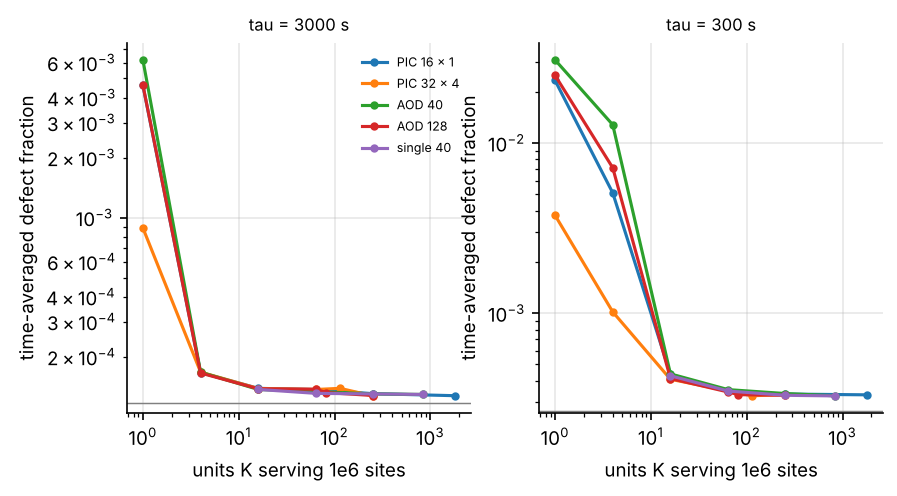
\includegraphics{../results/m29_figure.png}

\emph{Time-averaged steady-state defect fraction at 10\^{}6 sites
against the number of independent units K (zones of 10\^{}6/K sites),
cold steps, assembled start; left tau 3000 s, right 300 s. Grey line:
eps + T/(2 tau), the floor for zero latency.}

\hypertarget{4-limits}{%
\section{Limits}\label{concurrency-4-limits}}

\begin{itemize}
\tightlist
\item
  \textbf{Shared field.} K units must share one objective field. This is
  reported, not modelled. For the PIC, engines tile at 3.0 mm pitch with
  lenslets (module 24); for AOD pairs no tiling optics is designed or
  claimed.
\item
  \textbf{Loss model.} One loss model and one imaging cadence apply
  throughout. Zone boundaries are taken as hard; in practice, sites near
  a boundary could be served from either side.
\item
  \textbf{AOD model.} The crossed-AOD model is the row-wise lower bound
  of module 28.
\item
  \textbf{Statistics.} 2 to 6 seeds per case, about 600 losses per run.
\end{itemize}

\hypertarget{verification-notes}{%
\section{Verification notes}\label{concurrency-verification-notes}}

{\footnotesize
\begin{longtable}[]{@{}>{\raggedright\arraybackslash}p{0.257\dimexpr(\linewidth-8\tabcolsep)\relax}>{\raggedright\arraybackslash}p{0.129\dimexpr(\linewidth-8\tabcolsep)\relax}>{\raggedright\arraybackslash}p{0.123\dimexpr(\linewidth-8\tabcolsep)\relax}>{\raggedright\arraybackslash}p{0.491\dimexpr(\linewidth-8\tabcolsep)\relax}@{}}
\toprule\noalign{}
value & location & type & pointer \\
\midrule\noalign{}
\endhead
\bottomrule\noalign{}
\endlastfoot
defect fractions vs K, assembly times & Sec. 1, 3 & SIM &
results/m29\_ladder.json (review) \\
fast-step K = 1 and 4 at 10\^{}6 sites & Sec. 3 & SIM &
results/m29\_ladder\_fast.json (three seeds; review) \\
capacity per unit, peak tweezers & Sec. 1, 3 & SIM &
results/m29\_capacity.json (review) \\
power and channels vs K, smallest K & Sec. 1 & DERIVED &
results/m29\_hardware.json \\
floor eps + T/(2 tau) & Sec. 1 & DERIVED & docs/megascale.md Sec. 10 \\
demand 1,242/s (tau 3000 s), 4,242/s (300 s) & Sec. 1 & DERIVED & N
(1/tau + eps/(T\_img + t\_img)), cycle 0.11 s \\
units, timings, losses, per-tweezer powers & Sec. 2 & SIM / CHOICE /
SOURCE & docs/aod\_comparison.md \\
\end{longtable}
}
